\documentclass[10pt,twocolumn,letterpaper]{article}

\usepackage{cvpr}
\usepackage{times}
\usepackage{epsfig}
\usepackage{graphicx}
\usepackage{amsmath}
\usepackage{amssymb}

% Include other packages here, before hyperref.

% If you comment hyperref and then uncomment it, you should delete
% egpaper.aux before re-running latex.  (Or just hit 'q' on the first latex
% run, let it finish, and you should be clear).
\usepackage[breaklinks=true,bookmarks=false]{hyperref}

\cvprfinalcopy % *** Uncomment this line for the final submission

\def\cvprPaperID{****} % *** Enter the CVPR Paper ID here
\def\httilde{\mbox{\tt\raisebox{-.5ex}{\symbol{126}}}}

% Pages are numbered in submission mode, and unnumbered in camera-ready
%\ifcvprfinal\pagestyle{empty}\fi
\setcounter{page}{4321}
\begin{document}

%%%%%%%%% TITLE
\title{\LaTeX\ Author Guidelines for CVPR Proceedings}

\title{Amodal Instance Segmentation}

\author{Xiangyi Zhang\\
Supervisior: Xuming He\\
Shanghaitech University\\
%{\tt\small zhangxy9@shanghaitech.edu.cn}
%\and
%Supervisior: Xuming He\\
%Shanghaitech University\\
%{\tt\small zhangxy9@shanghaitech.edu.cn}
}


\maketitle
%\thispagestyle{empty}

%%%%%%%%% ABSTRACT
\begin{abstract}
   Common visual recognition task such as object detection, semantic segmentation
   are reaching high manurity. We now consider a different task of amodal segmentation
   which predicts the complete region of each object instance.  Amodal 
   segmentation plays an indispensable role in scene understanding, depth estimation,
   etc. We propose a novel part-based model  to infer amodal masks
   from a single RGB image, which then allows for an interative refinement of mask propopsals
   generated by a state-of-the-art Mask R-CNN variant finetuned for amodal instance 
   segmentation. We evalute our results on the publicly available COCO amodal dataset.
\end{abstract}

%%%%%%%%% BODY TEXT
\section{Introduction}
Recently, visual recognition tasks such as image classfication\cite{witten2016data,he2016deep}, object detection\cite{felzenszwalb2010object,sermanet2013overfeat}, edge detection\cite{arbelaez2011contour},
and semantic segmentation\cite{shotton2006textonboost,pinheiro2014recurrent,long2015fully}, have witnessed dramatic progress. While all of these progresses are in visible
field. We consider one challenge of predicting the invisible part. We take our inspiration
from the study of human visiual system. A remarkable advantage of human vision is the ease of interpolating
information of the invisible part, which in the end tranforms correct information to our brain and 
makes resonable decision. A particularly prominent example of this, and one on which we focus, is 
amodal instance segmentation.

Amodal instance segmentation, the ability of perceiving the whole of an object when it is partially occluded,
just like the basic form of mental vision system human has, which readily perceive partially occluded
objects and guess at their true shape.

There are three critical challenges to amodal instance segmentation. First, for occlusion, it is hard to 
predict scope of an incomplete object due to missing information and lack of prior knowledge. Secondly, there
exists large-scale variance on occlusion patterns. Thirdly, labeling such variant dataset is challenging
and expensive.

Based on these challenges, for occlusion, we adopt part-based representation instead of 
enumerating all occlusion patterns. We construct a refenrence set as a external memory bank which has complete maskes, providing the prior knowledge. In the meantime, the reference set without any amodal 
annotation also relieves the labeling burden.


\section{Related Work}
 \textbf{Instance segmentation}. Recent years witnessed a rapid progress of Convolutional Neural 
Network (CNN) based instance segmentation algorithms over conventional methods such as \cite{he2014exemplar}. 
Some of the most prominent examples include SDS \cite{hariharan2014simultaneous,hariharan2015hypercolumns,li2016iterative}, CFM \cite{dai2015convolutional}, MNC \cite{dai2016instance} and FCIS \cite{li2017fully}. 
These methods typically start with proposing a large pool of image regions in the form 
of either boxes or superpixels, and then make refinement to produce final segmentations
based on image features from deep neural networks. In contrast, there has also been work 
that does not rely on object proposals. For example, \cite{bai2017deep,Liang2015proposal,uhrig2016pixel} attempt to recover instance 
labels from semantic segmentation results. Other work has attempted to segment instances 
sequentially with a recurrent neural network \cite{romera2016recurrent}. Most relevant to ours are some of the 
recent work proposed for amodal perception of objects. Kar et al. \cite{kar2015amodal} propose to learn category\-specific
object size distributions for amodal bounding box prediction. Li et al.\cite{li2016amodal} proposes to predict amodal instance segmentations using the method from \cite{li2016iterative} with randomly overlaid occluders. In additioin, Ehasni et al. \cite{ehsani2017segan} propose a model for generating the appearance of the invisible parts of an object with a generative adversarial network. Of particular interest is the work from Zhu et al. \cite{premachandran2015pascal} that creates the largest publicly available amodal instance segmentation dataset based on a subset of the COCO dataset \cite{lin2014microsoft}. They established a solid baseline for class-agnostic amodal instance mask prediction. Their methods were built based on successful prior work including DeepMask \cite{pinheiro2015learning} and SharpMask \cite{pinheiro2016learning} for class-agonstic amodal segmentation. Although our method makes use of their dataset, we address the problem of class-specific amodal instance segmentation. We believe that it is essential to use strong top-down shape priors to guide the refinement process of bottom-up segmentation proposals. To our knowledge, our work is the first to consider the problem of amodal instance segmentation with both top-down and bottom-up visual cues.


\textbf{Amodal Instance Segemntation. }Recent works of instance segmentation are mainly on the visible field. Amodal segmentation focus on the invisible part. Research on amodal instance segmentation or semantic amodal segmentation has just started to emerge. Li and Malik \cite{ehsani2017segan} were the first to provide a method for amodal instance segmentation. In \cite{li2017scene}, Zhu et al. provide a new and pioneering
dataset COCO amodal for amodal instance segmentation based on images from
the original COCO \cite{lin2014microsoft} dataset. 



\textbf{Deep Voting. }
DeepVoting detects semantic parts of an object proposed by Zhang et al. They propose that all models should be trained without seeing occlusion while being able to transfer the learned knowledge to deal with occlusion.\cite{wang2017detecting} proposed a voting mechansim that combiens multiple laocal visual cues to detect semantic parts. The semantic meaning part s are still be detected even though some visual cues are missing due to occlusion. DeepVoting incroporates the robustness shown by \cite{wang2017detecting} into a deep network, and it adds two layers after the intermediate features of deep network. The first layer extracts the evidence of local visual cues, and the second layer perdorms a voting mechanism by utilizing the saptial relationship between visual cues and semantic parts.



\section{Model Setting}
The model setting preparing for the next two key branches contains pairset and rescaling.
\subsection{Pairset Setting}
We decide to take proposal data from Mask R-CNN as query set method,  which is image patch  $I_q$, size $W \times H$. And We adopt reference set as external memory bank  $I_r$, size $W \times H$. It plays the role of amodal annotation and amodal variation.
Then, we take query set and refenrence set as pairset data of input image patches($I_q, I_r$).
\subsubsection{Reference Set}

Reference set is composed of a set of paired instance image patches $I_r $ and corresponding mask patches $M_r$
cropped by {\bf ground truth bounding box}. Reference dataset
$D_{r} = \{I_r^{gt}, M_r^{gt}\}^{N_r}_{i=1}$, where $N_r$ is the size of refenrence set.

\subsubsection{Query Set}

Query set is composed of a set of paired instance image patches $I_q $ and corresponding mask patches $M_q$
cropped by {\bf proposal bounding box}, and mask patches $M_q^{gt}$ cropped by instance's {\bf ground truth bounding box}. Query dataset
$D_{q} = \{I_q^{prop}, M_q^{prop}, M_q^{gt}\}^{N_q}_{i=1}$, where $N_q$ is the size of query set.

\subsection{ScaleNet}
ScaleNet takes image patches $I_q$ or $I_r$ as input and predicts object scale $\hat{s}$, which is the 
ratio of the object bounding box short edge to the fixed long edge L. Its ground truth scale is denoted by $ s = \frac{min(H^{gt}, W^{gt})}{L}$,
where we set $L$ = 224 pixels.
   \begin{equation}
      \hat{s} = ScaleNet(I^{prop})
   \end{equation}


For query set data, after training of scalenet, the predicted ratio $\hat{s}$ is used to normalize the object to the desired size, which is, its short edge contains $L$ pixels.

   \begin{equation}
      \begin{split}
          I = Rescale(I^{prop};\hat{s})\in  {\mathbb{R}^{H\times W} },\\
          where \ H = \frac{H_p}{\hat{s}},  W = \frac{W_p}{\hat{s}} 
      \end{split}
   \end{equation}
   
   
For reference set, directly use its {\bf ground truth scale $s$ }for rescaling and denoted as $\tilde{D}_{ref} = \{I^i_r, M^i_r\}^{N_r}_{i=1}$.
 For query , we use {\bf predicted scale $\hat{s}$} for rescaling and denoted as $\tilde{D}_{q} = \{I^i_q, M^i_q\}^{N_q}_{i=1}$. 

After rescaling, we use threshold $\tau _{pos}$ and $\tau _{neg}$ to form positive and negtive pairs. For each query-ref pair, 
if their amodal ground truthh mask's overlap IoU$(M_r, M_q) \in (\tau_{pos},\tau_{neg})$, we will discard it. For reamined qualified
pairs, we assign classfication label by 

      $$ y=\left\{
      \begin{aligned}
      1  && if && IoU(M_r, M_q) \geq \tau_{pos} \\
      0  && if && IoU(M_r, M_q) \leq \tau_{neg}
      \end{aligned}
      \right.
      $$
      
      
The goal of ScaleNet is to put query and reference data into the same scale size.


\section{Model}
We design a mask transfer pipeline shown in Figure \ref{fig:pipeline}. The key idea is to find the most similar complete mask. Then go through the part-based voting branch to find the correct position for mask transfer.  We propose a system to vote a heatmap which is the probable center of query and reference data, then find the most similar reference mask center-aligned to query and get the prediction of query's complete mask.  

	\begin{figure*}[h]
	\begin{center}
		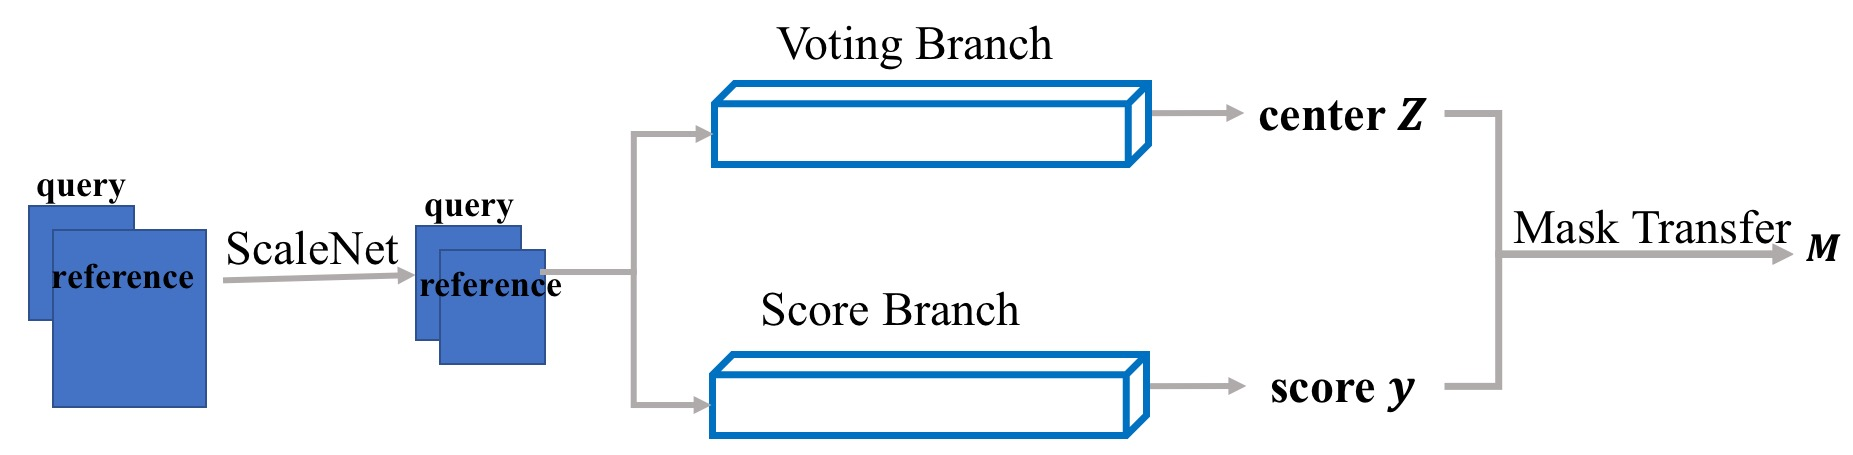
\includegraphics[width=0.8\textwidth]{pipeline.png}
		\caption{The mask transfer pipeline is to find the most similar complete mask for the correct position for mask transfer. We utilize voting and score these two branches. }
		\label{fig:pipeline}
	\end{center}
\end{figure*}
\subsection{Voting Branch}
In voting branch, first we take query and reference image patches as input pairset($I_q, I_r$), and go through  a voting layer to vote the center of an object instance in feature map space\cite{wang2015unsupervised,zhang2018deepvoting},  shown in Figure \ref{fig:vote}
\begin{figure*}
   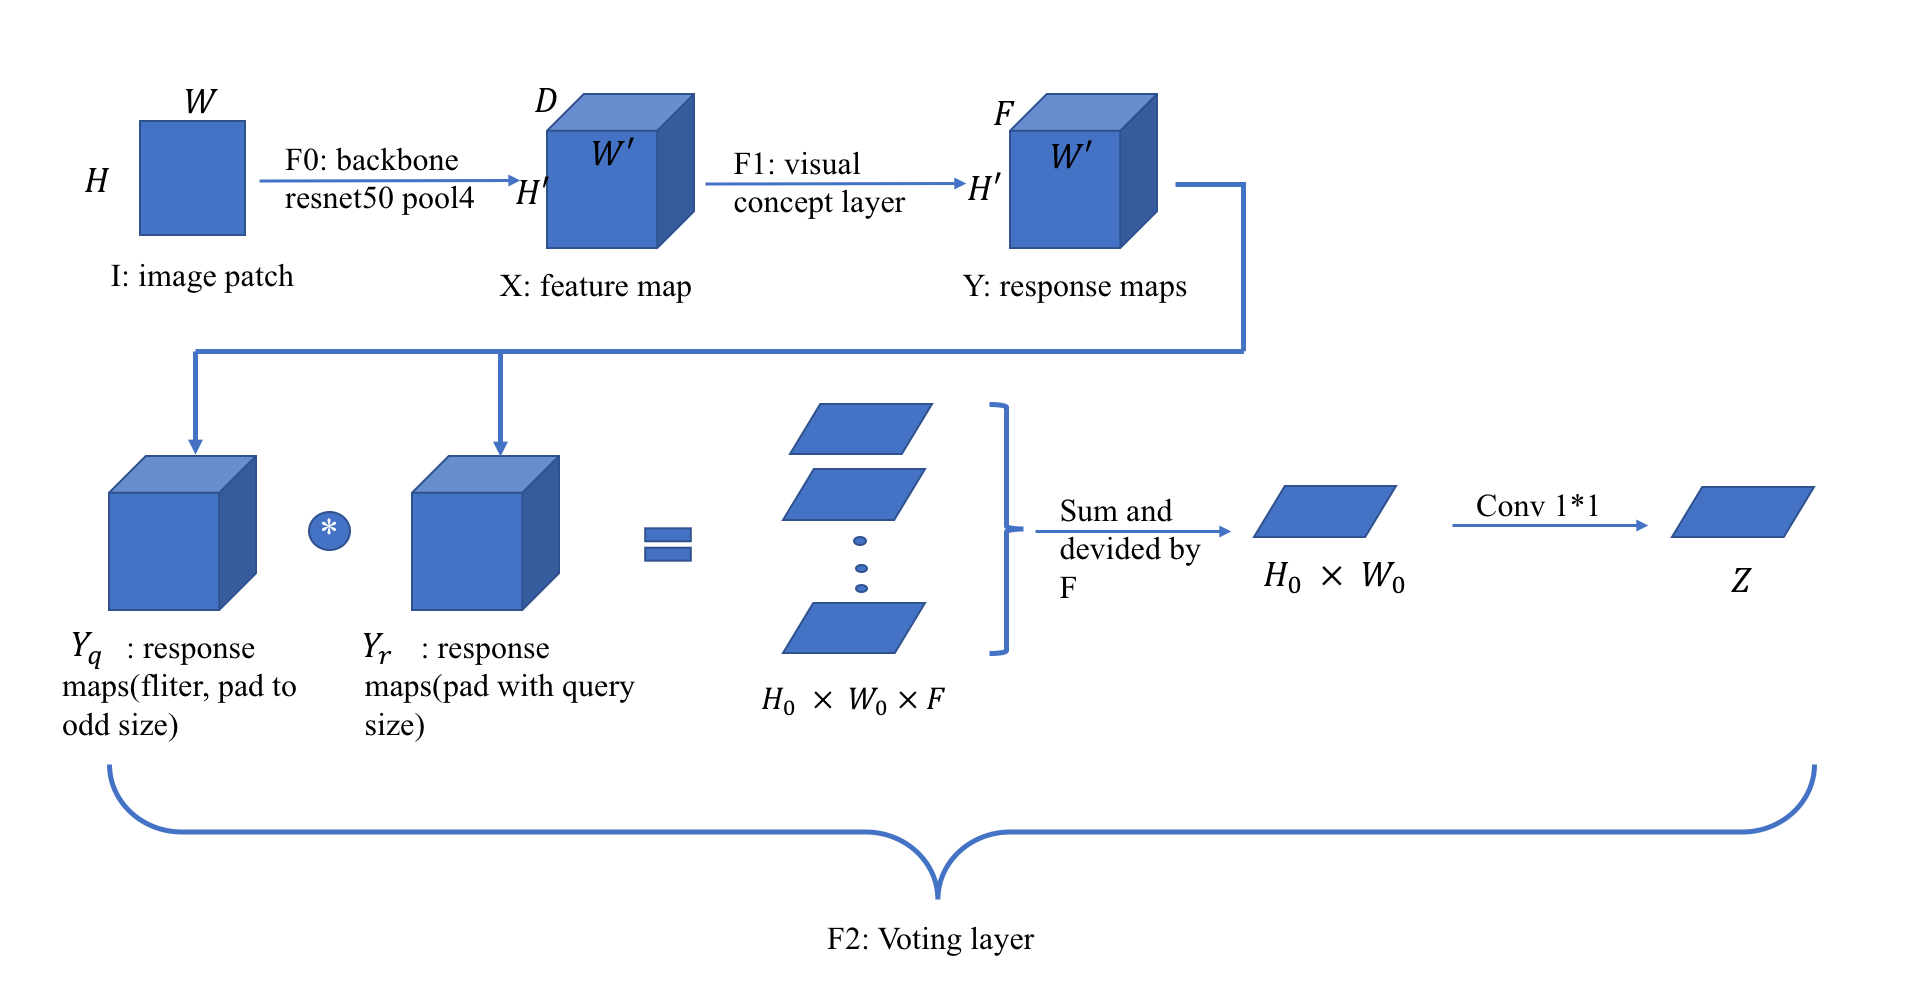
\includegraphics[width=1\textwidth]{vote.png}
   \caption{\textbf{Voting Branch}. We first go through  $F_0$ :Backbone of resent50 and utilize a visual concept(VC) layer$F_1$ to generate response maps which represented in lower left quarter as $Y_q$: response map of query set and $Y_r$ : response map of refenrence set. These two images  both highlight in left and upper corner which means VC layer learns consistent semantic meaning there.  Then go through a ConvNet to get the predicted center $z$: voting heatmap, size $W' \times H' $. }
   \label{fig:vote}
\end{figure*}


\subsubsection{Visual Concept layer}
This layer outputs response maps, which can be described as follows:

   \begin{equation}
      Y = f_1(X;w1,\overline{w})
   \end{equation}
   where $X$ is feature map of image patch, parameter $w_1$ is the convolutional weight parameter for visual concept, size $1 \times 1\times F $, and $\overline{w}$ is the convolutional parameter for visual concept layer, which measures how important of each visual concept.

\subsubsection{Voting layer}
Take response maps $Y$ as input, this layer outputs object's voting heatmaps $Z$, whcih is the predicted center while ground truth is $Z^*$. 
\begin{equation}
   Z = f_2(Y;w_2)
\end{equation}
Here $Y$ consists of a pairset $(Y_q, Y_r)$, since query and reference set they all get through the VC layer
and generate the response maps. We utilize $Y_q$ as filter to convolute with $Y_r$, which pads with query size. 
So the $H'_r = H_r + 2 \times H_q $. We use MSE loss between $Z$ and $Z^*$. $w_2$ is the weight parameter for voting layer, size $k_2\times k_2 \times F$.
\begin{equation}
   Loss = MSE(Z, Z^*)
\end{equation}




\subsection{Score Branch}
Based on voting branch, our goal in score branch is to find the most similar reference to query. So we use similarity score to measure how similar
between current query image and reference image. If we choose the most similar reference mask, and center aligned to query mask's center, we can get amodal mask.

Score branch is similar to vote branch but add one classfication which represented in Figure \ref{fig:score}. Here we use $Binary\ cross\ entropy$ loss for mask similarity score, $y^*$ is ground truth of score. $Mean\ Square\ Error$ loss for regularization and coefficient is $\varepsilon$.
\begin{figure*}
   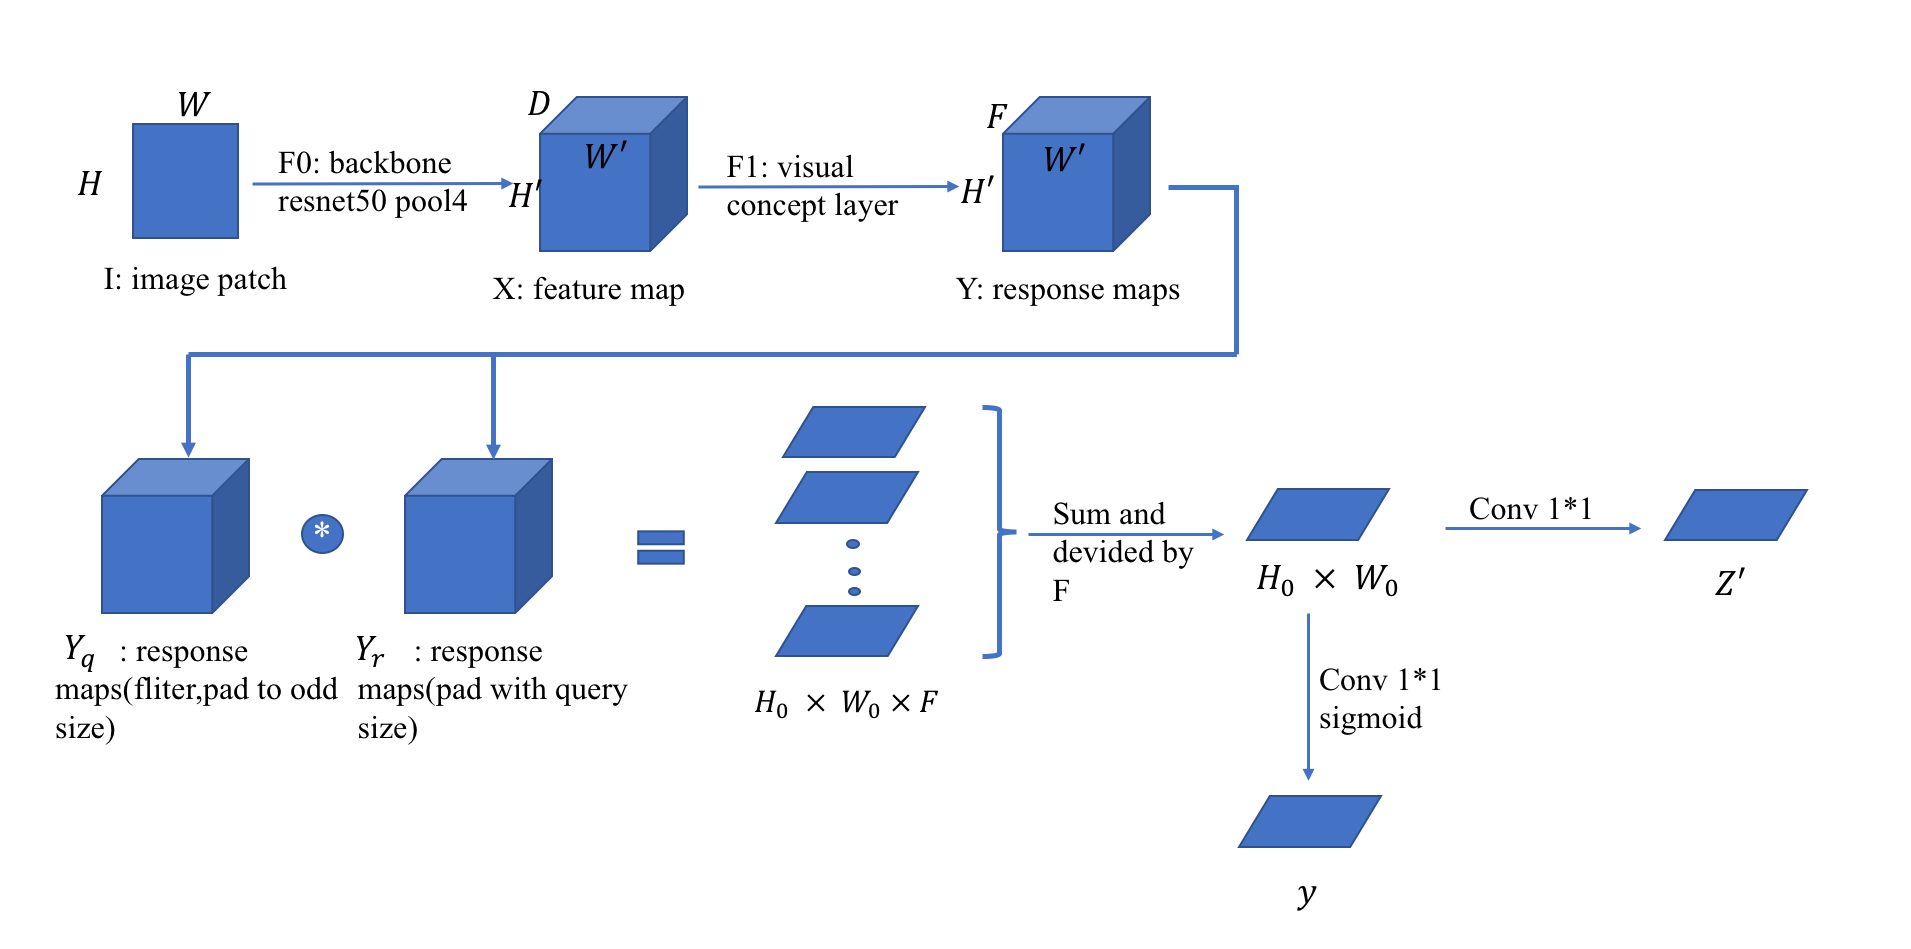
\includegraphics[width=1\textwidth]{score.png}
   \caption{Score Branch. $y$ is the similarity score between query and reference, $z'$ is the voting center for votng branch but as regularization.}
   \label{fig:score}
\end{figure*}
\begin{equation}
   Loss = BCE(y,y^*) + \varepsilon * MSE(Z', Z^*)
\end{equation}
\subsection{Mask Transfer}
We use a non-parametric way to transfer reference masks to query mask. We choose score top1 
mask from score branch and center-aligned to the query incomplete mask from voting branch, which 
finally get complete mask.



\section{Experiment}

We perform a  comparision of Mask R-CNN to the state of the art with our method on COCO amodal dataset. We report the standard COCO metrics including AP(averaged over IoU thresholds) evaluting mask IoU.  

\subsection{Dataset}
Our dataset contains query dataset and reference set: COCO amodal dataset and Cityscape dataset in  Table \ref{tab:dataset}. And our method now only applies on car category. 

\begin{table}[h]
   \begin{center}
		
      \begin{tabular}{lll}
      \multicolumn{3}{c}{Annotation} \\
      \hline
      Dataset  &    coco amodal     &  cityscape \\
      \hline
      Annotation & only car label & only car label\\
      image & train:228 val: 144 & 320\\
      %annotation & train:228 val: 144 & 3080 \\
      categories & 1: car & 1: car\\ 
   
      \hline

      \end{tabular}
      
   
   \end{center}
   \caption{We train our baseline of 228 train image in COCO amodal dataset, and 320 train image chose from
   Cityscape dataset as our refenrence set. And 144 val image from COCO amodal dataset.}
      \label{tab:dataset}
\end{table}

while training, we consider query and reference set data as pairset. Here is our training pairset-data. We compare Mask R-CNN to the state-of-the-art  methods in amodal segmentation in Table \ref{tab:data number}.

\begin{table}[h]
	\begin{center}
		
		\begin{tabular}{llll}
			\multicolumn{4}{c}{Data Number} \\
			\hline
			train\_{pos} & train\_{neg}&val\_{pos} & val\_{neg} \\
			\hline
			30614 & 28532 & 18638 & 15529 \\
		
		\end{tabular}
		
	\end{center}
	\caption{Negetive maskIoU
		threshold is 0.55, positive maskIoU threshold is 0.75}
\label{tab:data number}
\end{table}



\subsection{Voting and score Result}
Voting branch give us center-aligned result, which predicts object center. And here we use two metrics: $mindelta$ and $rgood(0.1)$ to evalute our result of voting in Table \ref{tab:vote_result}. Score branch predicts similarity between query and reference set while evaluating in three accuracy metrics: $pos\_acc$, $neg\_acc$ and $acc\_all$ in Table \ref{tab:score_result}. Finally,
the visualization results in Figure \ref{fig:response_vis} shows response maps through VC layer. Figure \ref{fig:vote_vis} presents our voting branch result. And score branch's result is in Figure \ref{fig:score_vis}.
\begin{table}[h]
	\begin{center}
		\begin{tabular}{ll}
			\multicolumn{2}{c}{Voting Branch} \\
			\hline
			mindelta &  0.067   \\
			\hline
			rgood(0.1)& 0.76  \\
		\end{tabular}

	\end{center}
	\caption{we compute each detla between voting result and ground truth. $ mindetla $ means we get minimum delta from the best epoch. $ rgood(0.1) $ means relative error of both x and y axis is within 10\%. }
	\label{tab:vote_result}
\end{table}

\begin{table}[h]
	\begin{center}
		\begin{tabular}{ll}
			\multicolumn{2}{c}{Score Branch } \\
			\hline
			pos\_acc &  0.742   \\
			\hline
			neg\_acc &  0.847   \\
			\hline
			acc\_all & 0.793   \\
		\end{tabular}

	\end{center}
	\caption{ $pos\_acc$ and $neg\_acc$ show positive and negative pairs' accuracy. The accuracy of positive and negative are balanced.}
	\label{tab:score_result}
\end{table}


	\begin{figure}[h]
		\begin{center}
		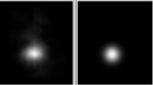
\includegraphics[width=0.258\textwidth]{vote_out2.png}
		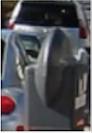
\includegraphics[width=0.1\textwidth]{vote_img.png}
		\caption{From left to right: Voting result, voting ground truth, query image patch. Voting result is close to voting target which proves
		voting accuracy. The voting result heatmap shows the direction and distance relative to voting target. When voting result is below the central point, it means our real center in image patch is above the central point.}
		\label{fig:vote_vis}
	\end{center}
	\end{figure}



\begin{figure}
	\begin{center}
		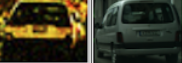
\includegraphics[width=0.3\textwidth]{img_patch.png}
		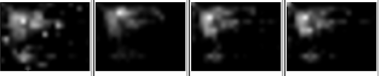
\includegraphics[width=0.3\textwidth]{query_resp2.png}
		
\includegraphics[width=0.3\textwidth]{ref_resp.png}
		\caption{First row shows query image patch on the left and ref set on the right. Response map of query and ref are on the second and 
			third row. Response maps generated from VC layer indicates some semantic parts in different maps. Second row and third row show that VC layer learns the consistent semantic meaning of query and ref, so they highlight on the same parts.}
			\label{fig:response_vis}
		\end{center}
		
	\end{figure}

\begin{figure}[h]
	\begin{center}
		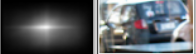
\includegraphics[width=0.3\textwidth]{score_out.png}
		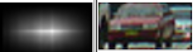
\includegraphics[width=0.3\textwidth]{score_out2.png}

		\caption{First column shows score branch regularization result, and image patches are on the right. One car generates one highlight heatmap while two ouputs two highlight points.}
		\label{fig:score_vis}
	\end{center}
	
\end{figure}
\subsection{Mask Transfer }
The key idea of mask transfer is to find the most similar complete mask of reference and put into the query's correct position. The visualization is shown in Figure \ref{fig:result} . In our result, we use two metrics: meanIoU and mAP, result shown in Figure \ref{tab: AP}. The analysis of lower AP is shown in Figure \ref{tab:analysis}The key componet matching need further improved, we could use feature transfer in our feature work to get better results.

\begin{figure*}[tpb]
	\begin{center}
		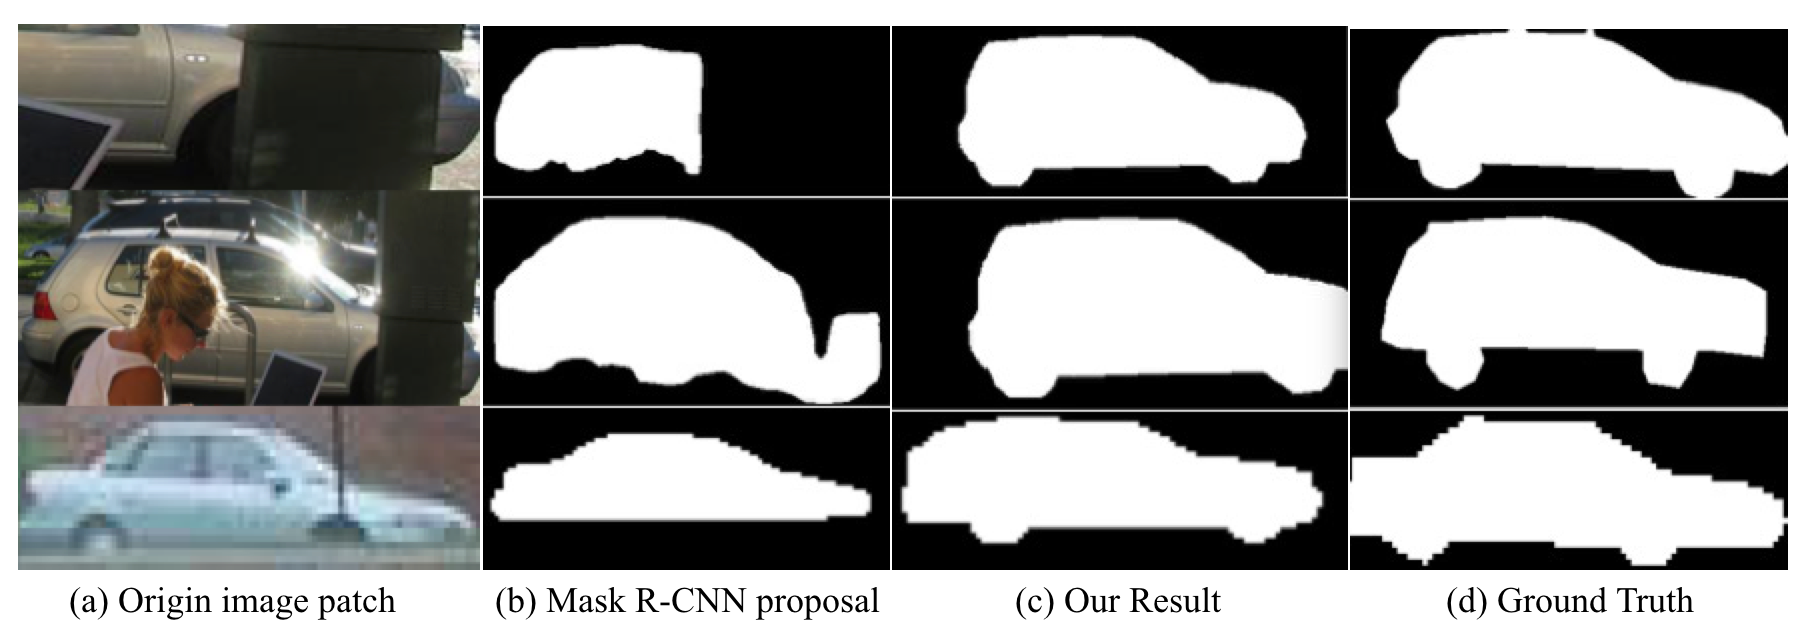
\includegraphics[width=0.8\textwidth]{result.png}
		
		\caption{First colume(a) shows the origin image patches. Second column(b) shows Mask R-CNN proposals which is incomplete while third column(c) is the predicted complete mask for our method. And the last(d) is the ground truth mask.}
		\label{fig:result}
	\end{center}
	
\end{figure*}
\begin{table}
	\begin{center}
		\begin{tabular}{lll}
			\multicolumn{3}{c}{Mask Transfer} \\
			\hline
			  &  meanIoU & AP   \\
			\hline
			Mask R-CNN & 0.5216 &  46.5 \\
			Our Method & 0.6970 & 40.2 
		\end{tabular}
	\end{center}
	\caption{$meanIoU$ means IoU between predicted mask and  ground truth mask. Our method improves meanIoU but get AP result not so good.}
\label{tab: AP}
\end{table}


\begin{table}
\begin{center}
	\begin{tabular}{llllll}
		\multicolumn{6}{c}{Analysis for lower AP} \\
		\hline
		IoU\_thres&  0.5 & 0.65 & 0.75 & 0.9 & meanAP \\
		\hline
		Mask R-CNN & 75.3 & 66.2 & 49.8 & 10.7 & 46.5 \\
		Our Method & 84.4 &68.9  & 25.6 & 0.0 & 40.2 
	\end{tabular}
\end{center}
\caption{We get better AP in lower IoU thresholds but worse in higher IoU thresholds. Maybe there is some weakness in VC layer-based matching, it could be our future work to consider an alternative matching strategy to fix this problem.
}
\label{tab:analysis}
\end{table}


\section{Conclusion}
We proposed a Mask transfer system to solve the amodal instance segmentation problem.
 We design a part-based voting and score system and build an external dataset to do the mask transfer.
The results show that the prediction of amodal and in particular invisible masks is a difficult task that needs further research.


{\small
\bibliographystyle{ieee}
\bibliography{egbib}
}

\end{document}